\newpage
\section{Anhang}
\subsection{Anhang 1}
\label{sec:Anhang1}
\begin{table}[htbp]
\begin{center}
%\caption[Vergleich externes- und internes Rechnungswesen]{Vergleich externes- und internes Rechnungswesen}
Vergleich externes- und internes Rechnungswesen
\includegraphics[width=1\textwidth]{Images/VergleichIntExt.png}
\label{abb1}
{\footnotesize In Anlehnung an: \cite{Lojewski2001}, S. 6}
\end{center}
\end{table} 
\newpage
\subsection{Anhang 2}
\label{sec:Anhang2}
\begin{table}[htbp]
\begin{center}
%\caption[Arten der Ergebnis- und Marktsegmentrechnung]{Arten der Ergebnis- und Marktsegmentrechnung}\label{tbl2}
Arten der Ergebnis- und Marktsegmentrechnung
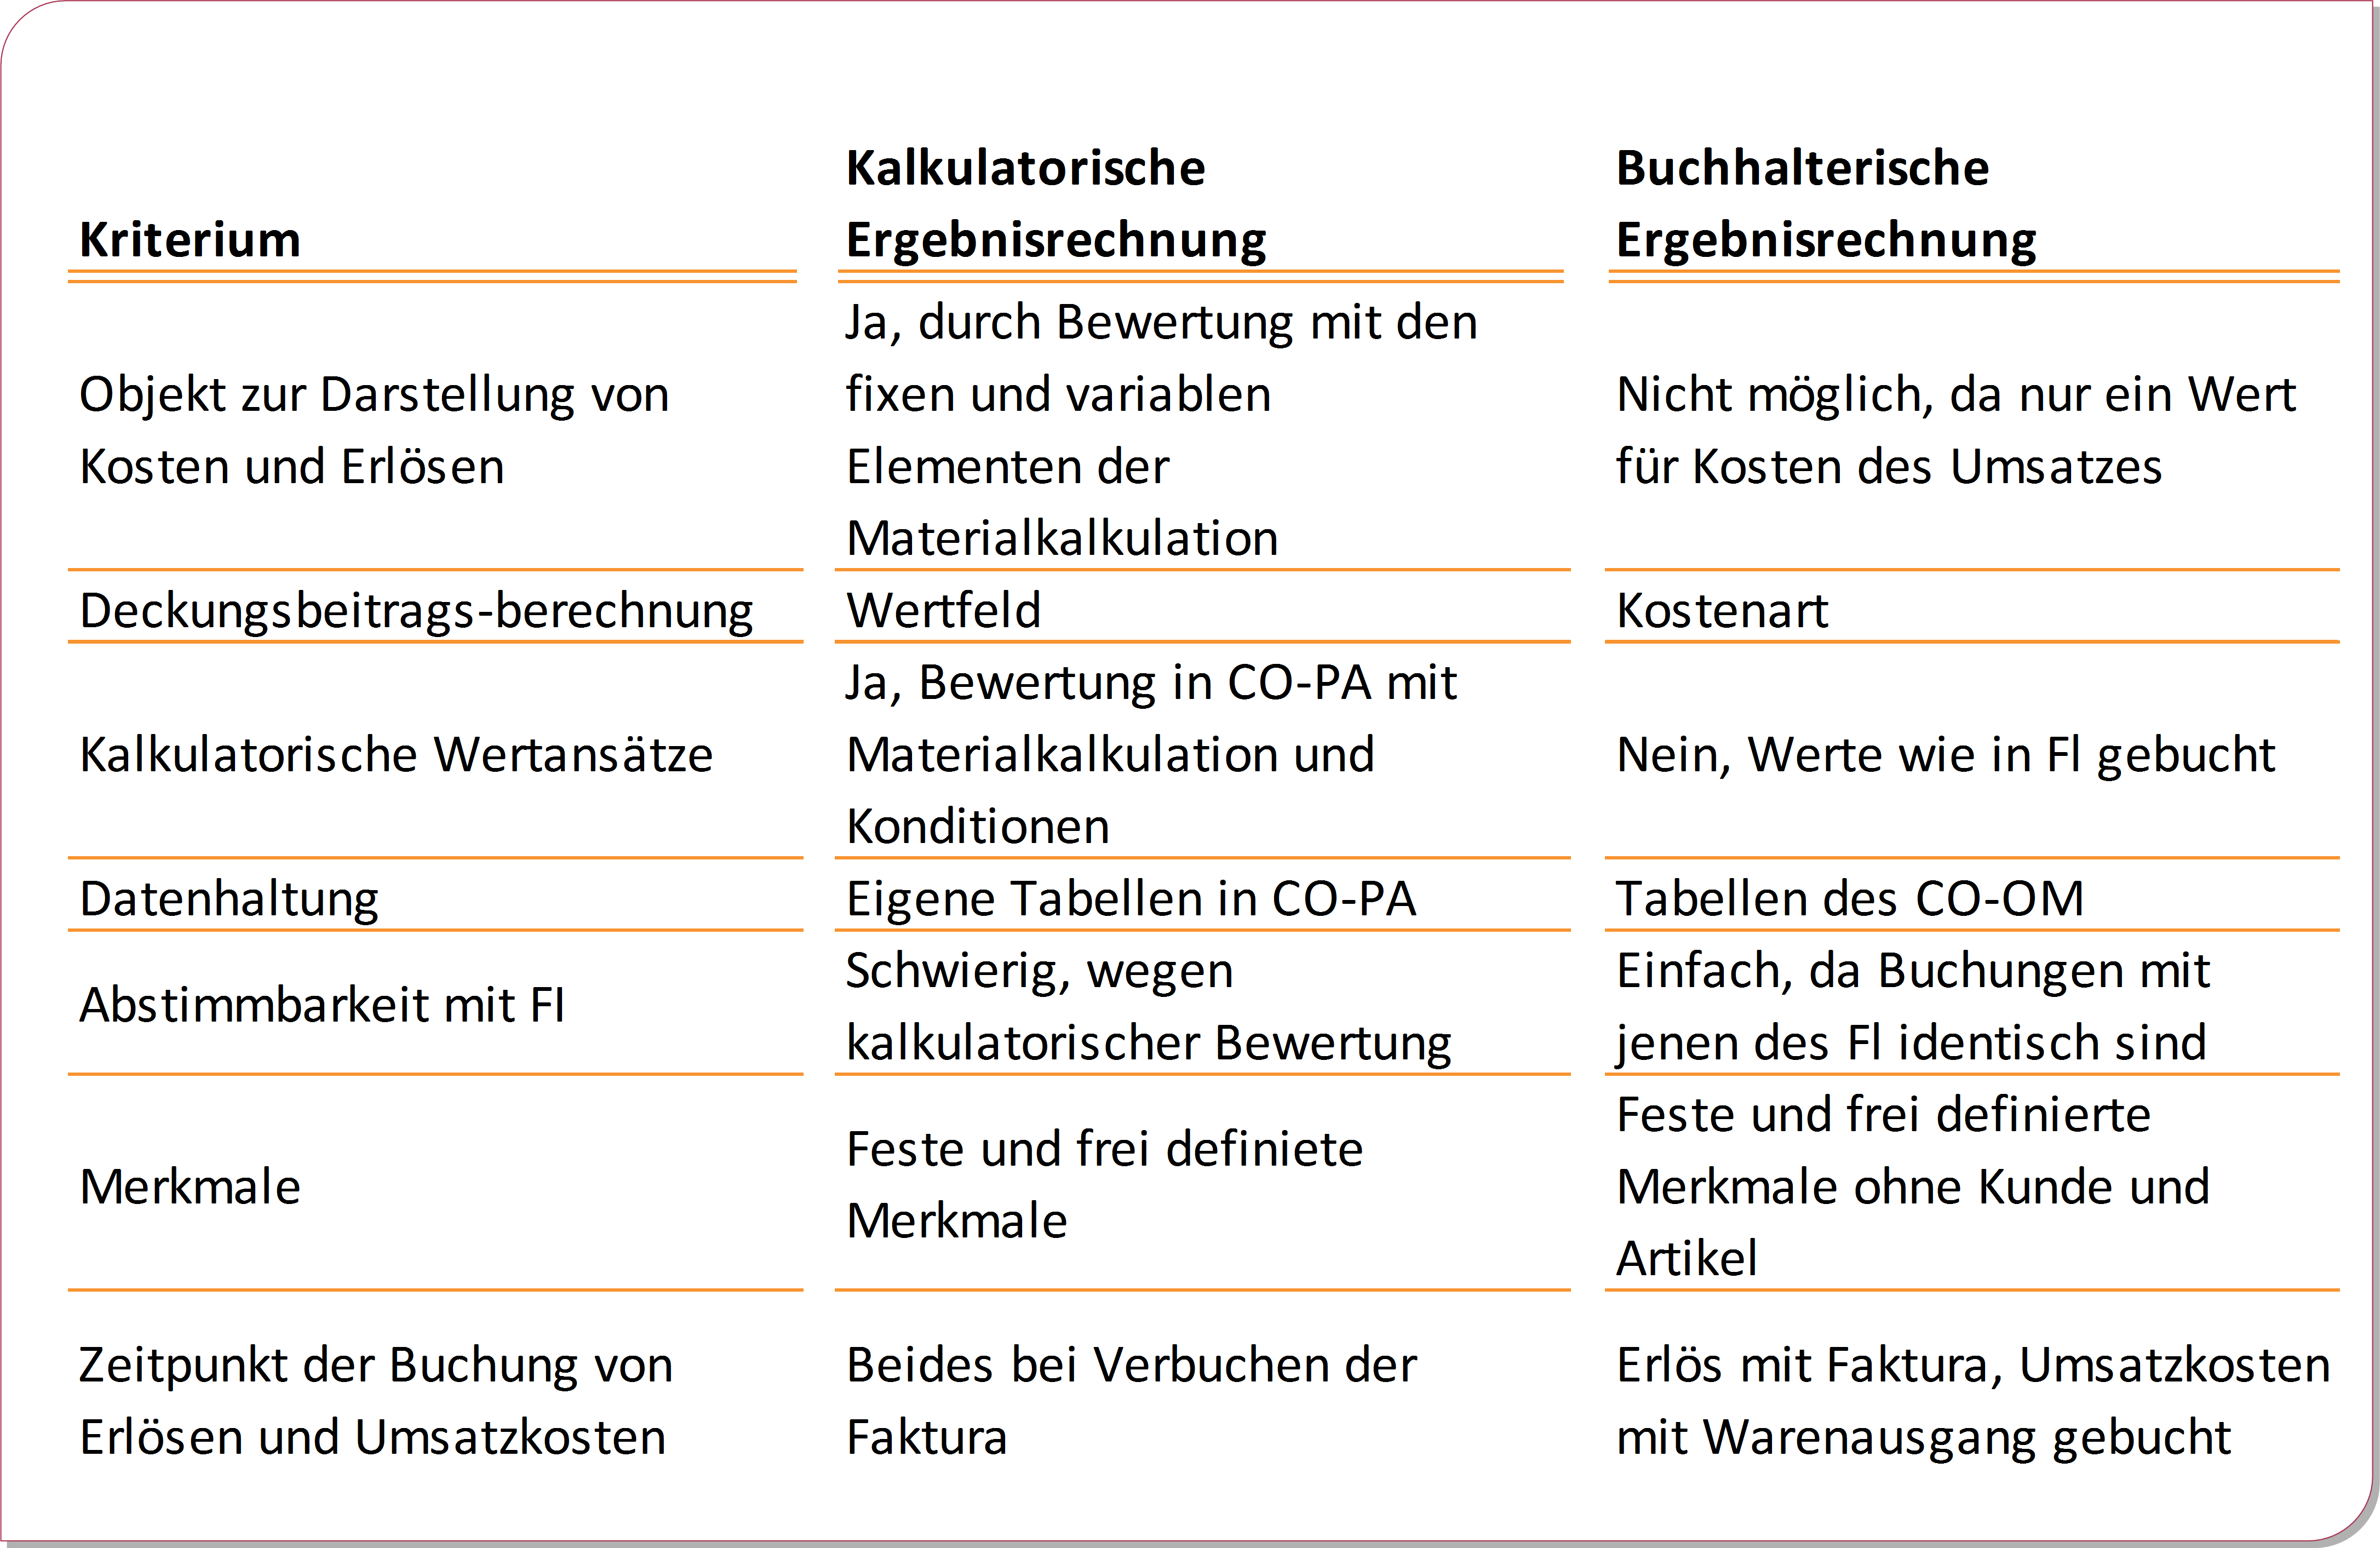
\includegraphics[width=1\textwidth]{Images/ergebnisrechnung.png}
{\footnotesize In Anlehnung an: \cite{Klein2010}, S. 275}
\end{center}
\end{table}